\subsection{Common Pages}

\noindent The common pages are accessible to all users and handle shared functionalities such as authentication, profile management, library access, and community interaction.

\subsubsection{Login / Logout}

\noindent The "Login / Logout" page provides users with secure access to the platform through multiple authentication methods, including email login and Single Sign-On (SSO) options.

\begin{figure}[H]
    \centering
    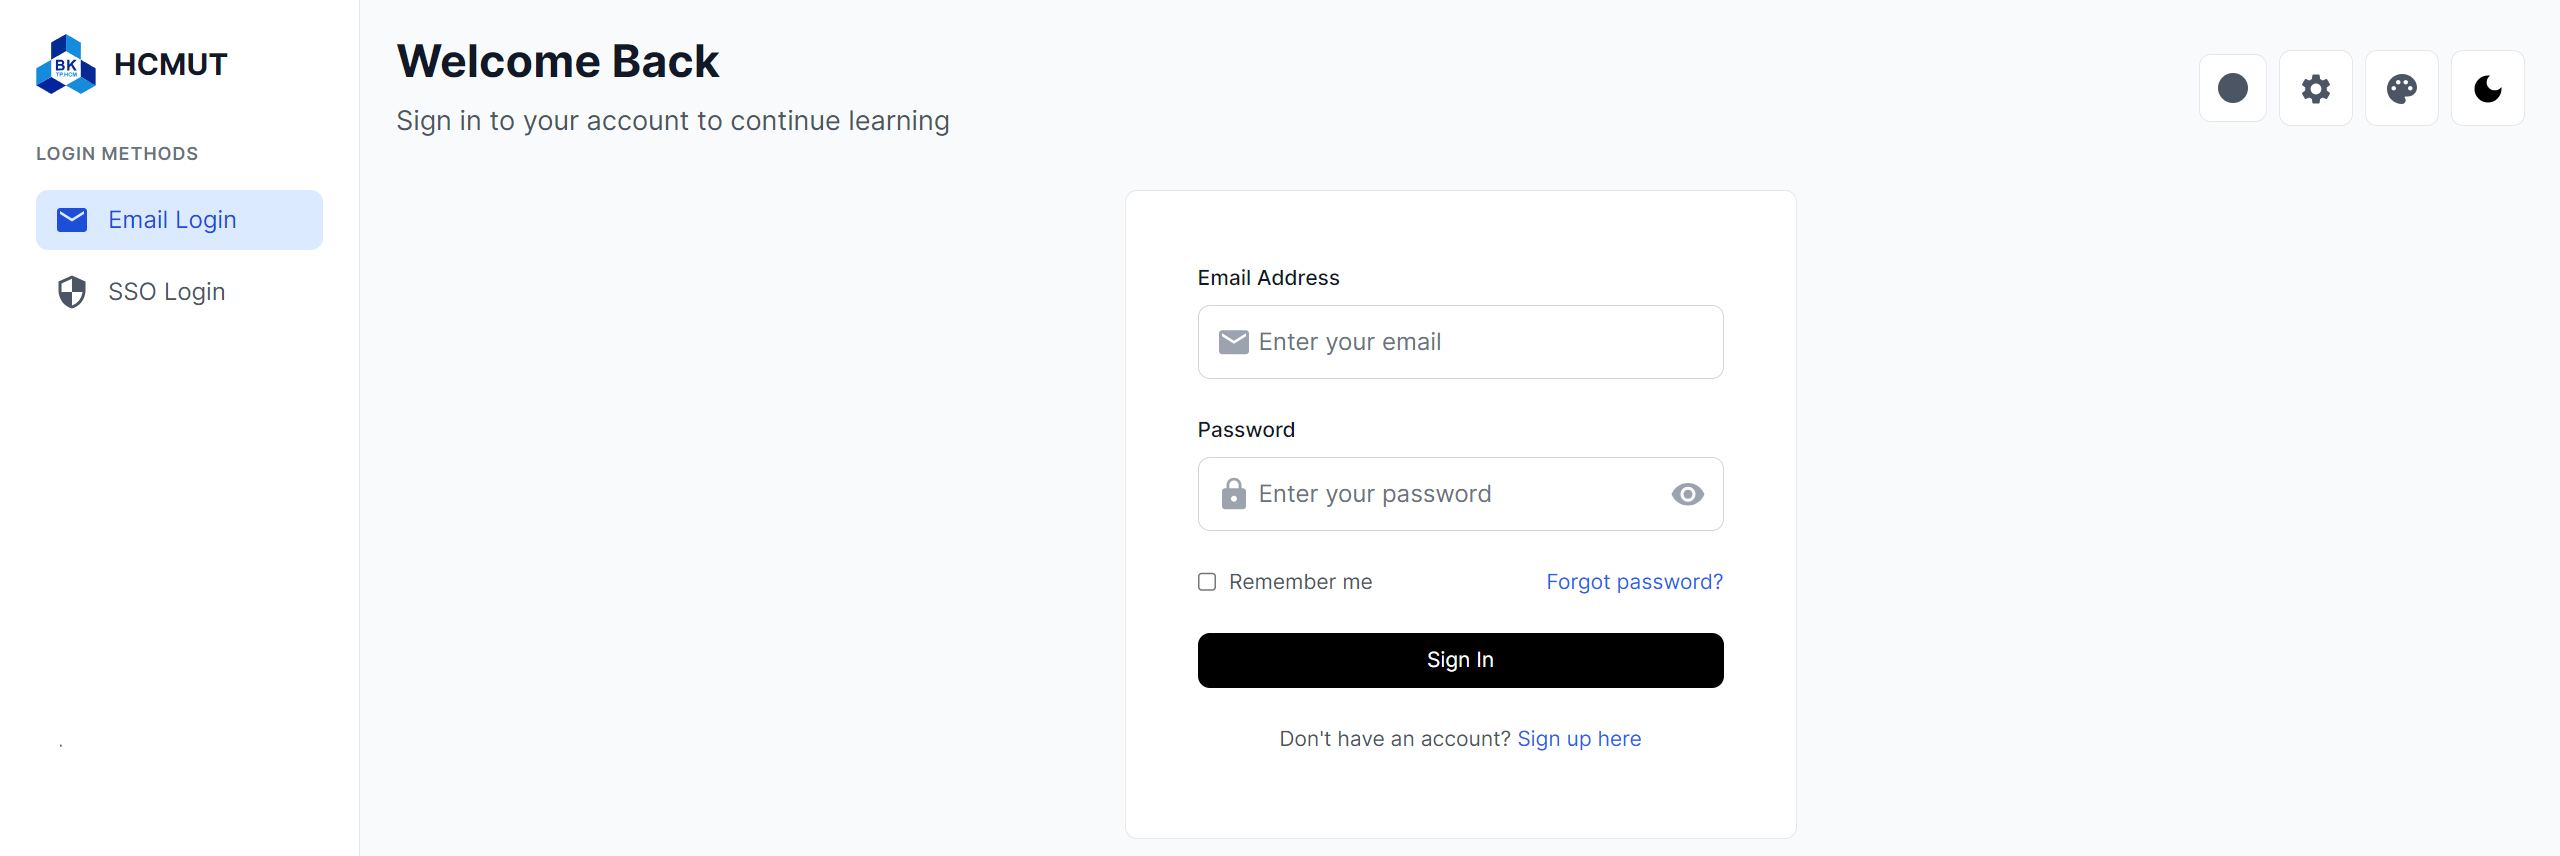
\includegraphics[width=\textwidth]{graphics/chapter2/common/login_desktop_overall.png}
    \caption{Login Page Overview (Desktop)}
    \label{fig:login_desktop_overall}
\end{figure}

\paragraph{General Overview (Desktop)}
The desktop interface features a clean, modern design with a left sidebar for login methods and a central content area for the login form.

\subsubsection{Profile Management}

\noindent The "Profile Management" page allows users to view and edit their personal, educational, and career information, as well as details about themselves, including interests and skills.

\begin{figure}[H]
    \centering
    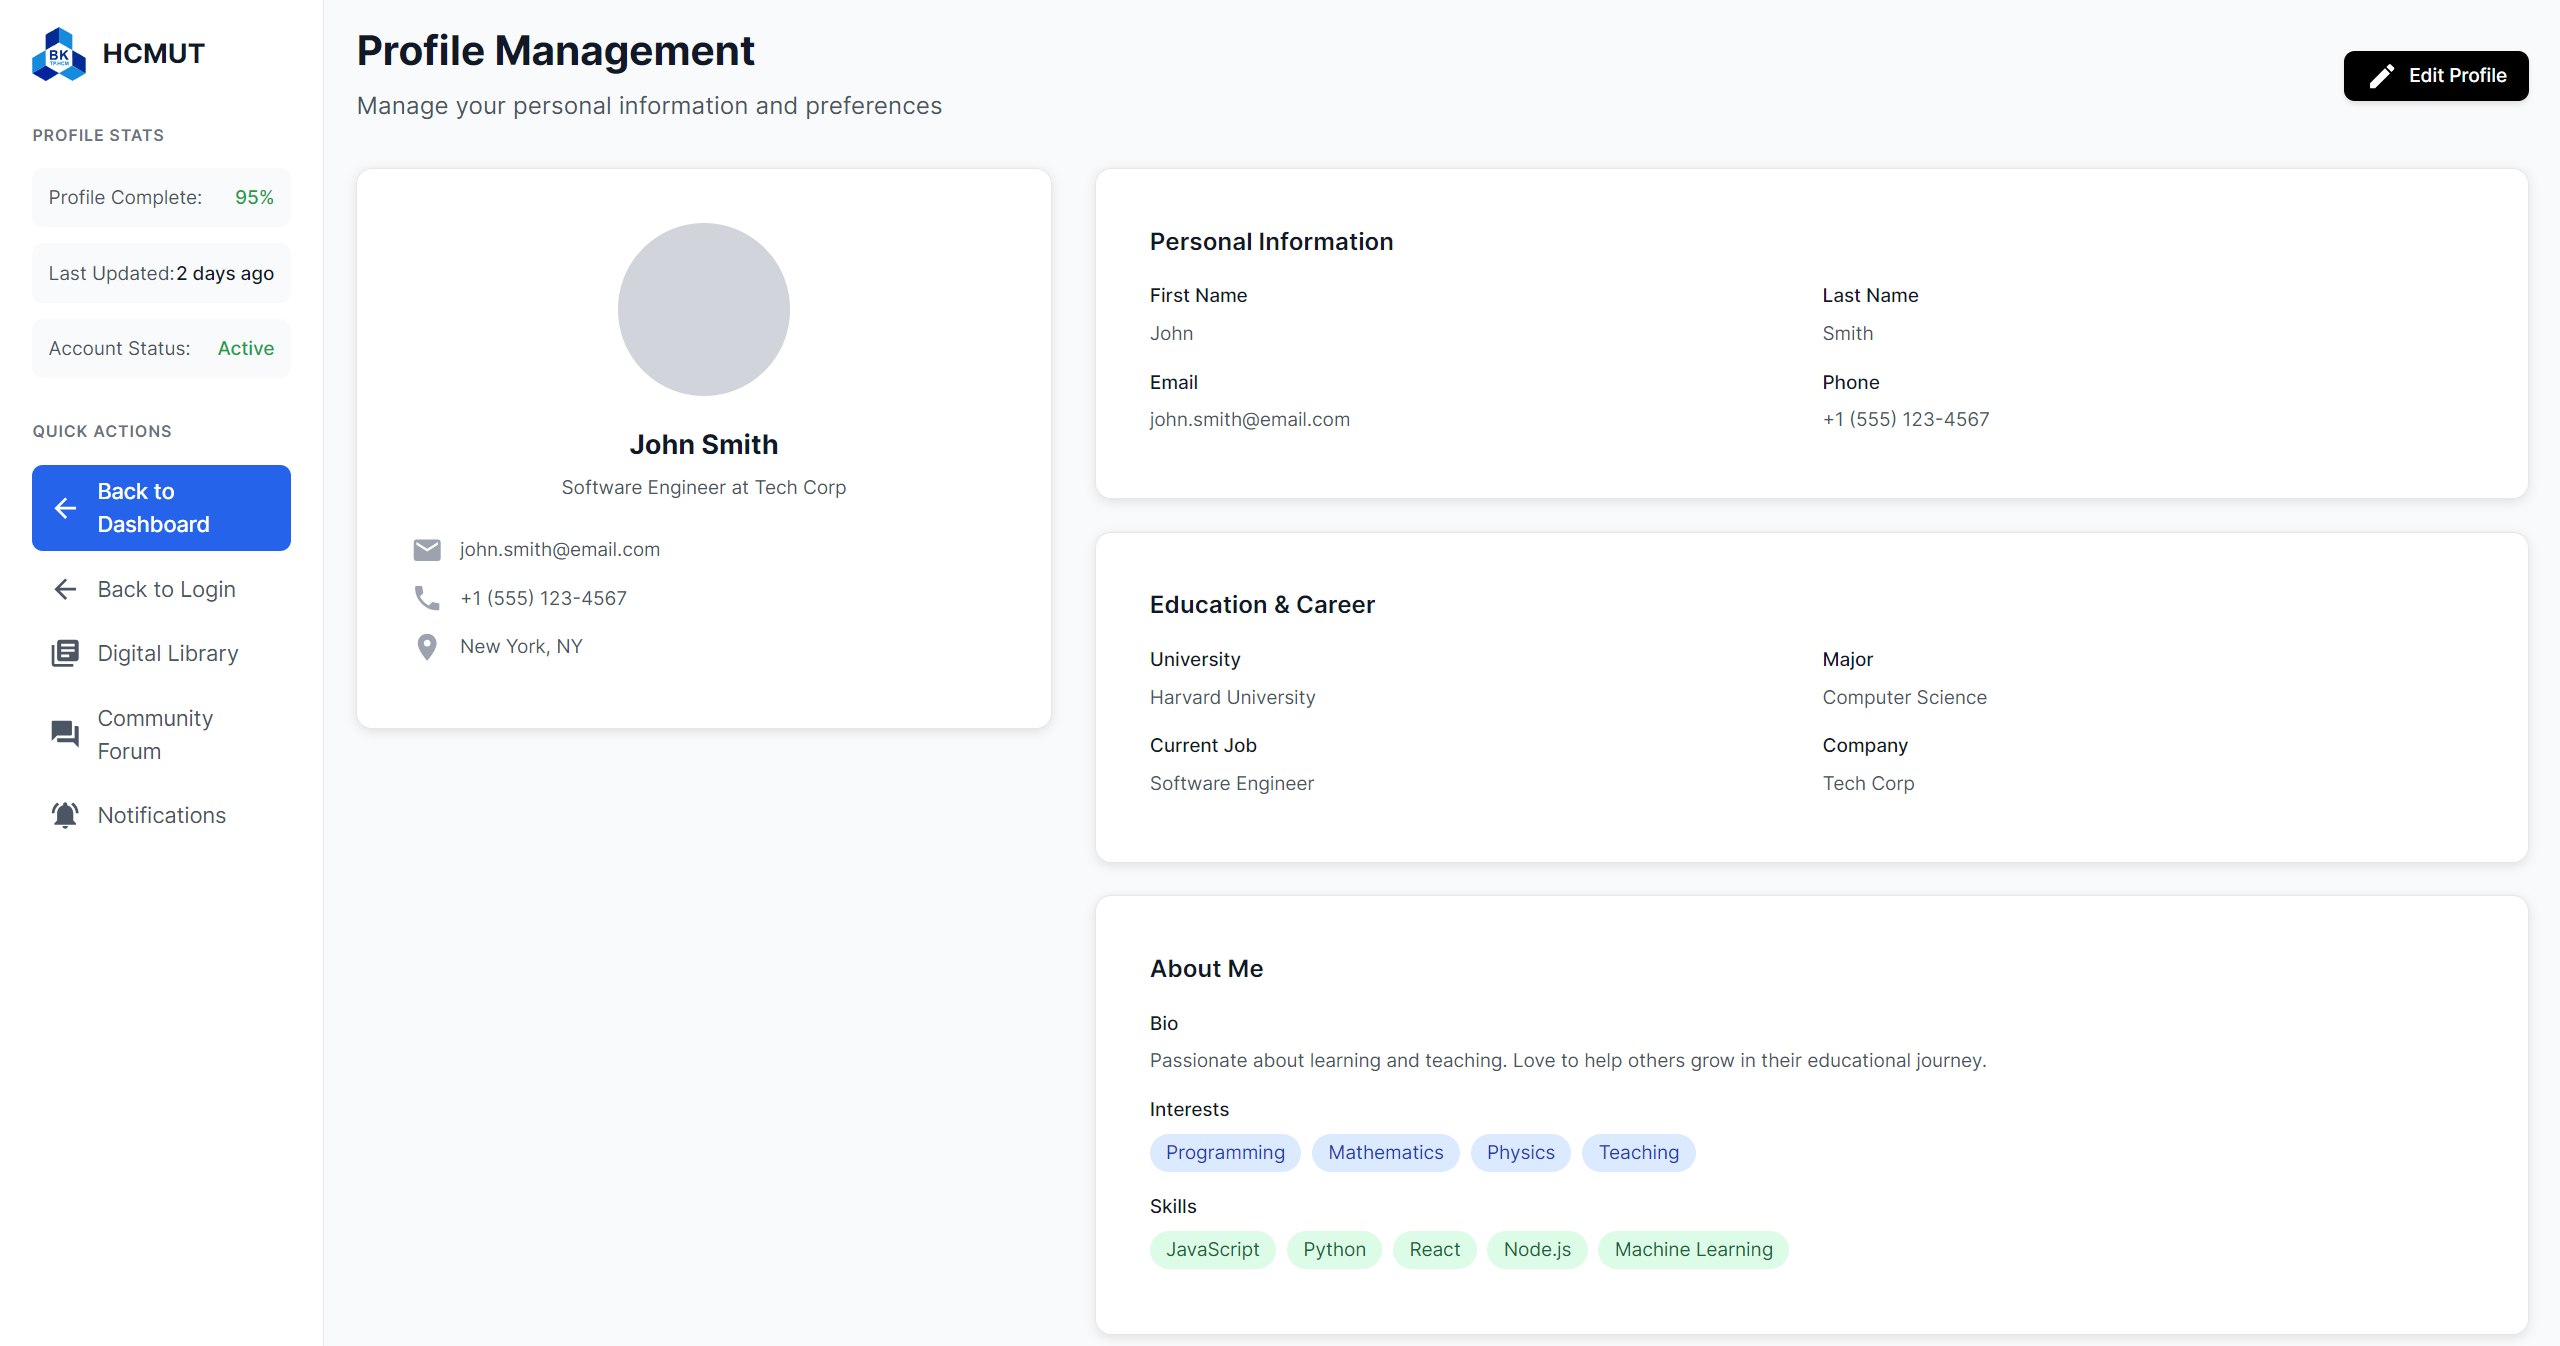
\includegraphics[width=\textwidth]{graphics/chapter2/common/profile_management_desktop_overall.png}
    \caption{Profile Management Page Overview (Desktop)}
    \label{fig:profile_management_desktop_overall}
\end{figure}

\paragraph{General Overview (Desktop)}
The desktop interface features a clean, modern design with profile statistics, user information, and editable form sections. 

\subsubsection{Digital Library Access}

\noindent The "Digital Library Access" page provides users with a centralized platform to search, access, and manage educational resources, including books, articles, and learning materials.

\begin{figure}[H]
    \centering
    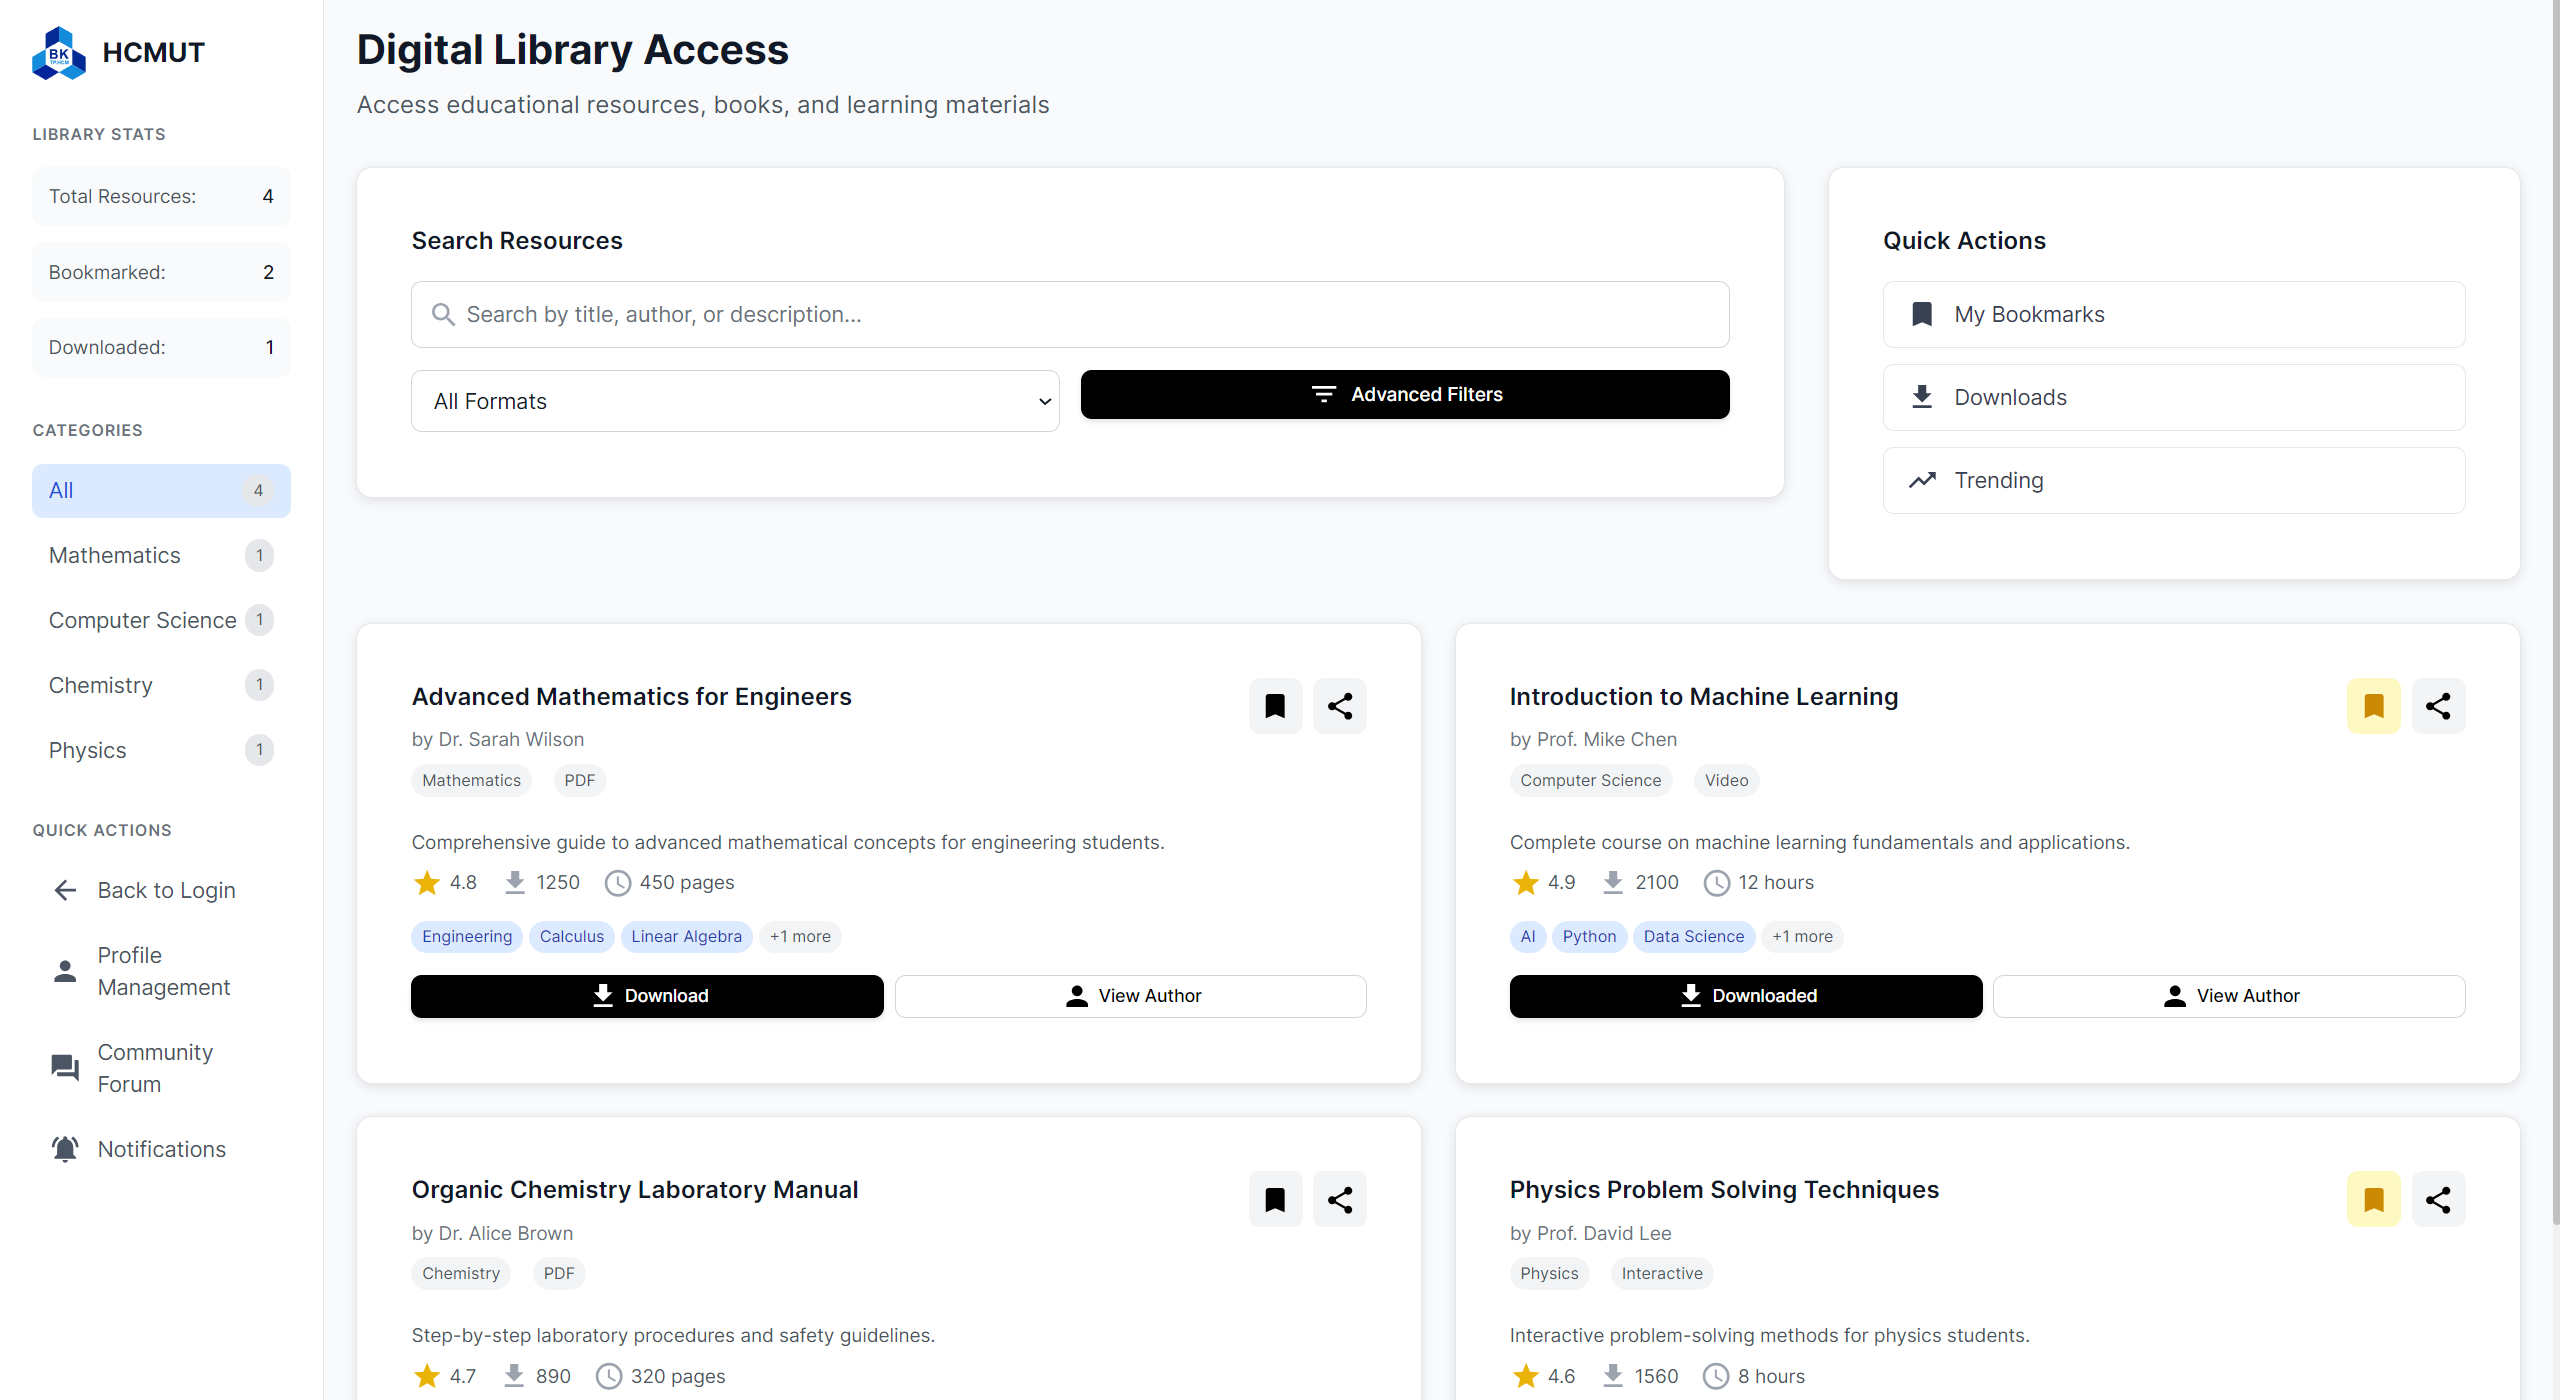
\includegraphics[width=\textwidth]{graphics/chapter2/common/digital_library_desktop_overall.png}
    \caption{Digital Library Access Page Overview (Desktop)}
    \label{fig:digital_library_desktop_overall}
\end{figure}

\paragraph{General Overview (Desktop)}
The desktop interface features a clean, modern design with library statistics, search functionality, category filters, and quick action buttons.

\subsubsection{Online Community Forum}

\noindent The "Online Community Forum" page serves as a central hub for users to connect, learn, and share knowledge within the community.

\begin{figure}[H]
    \centering
    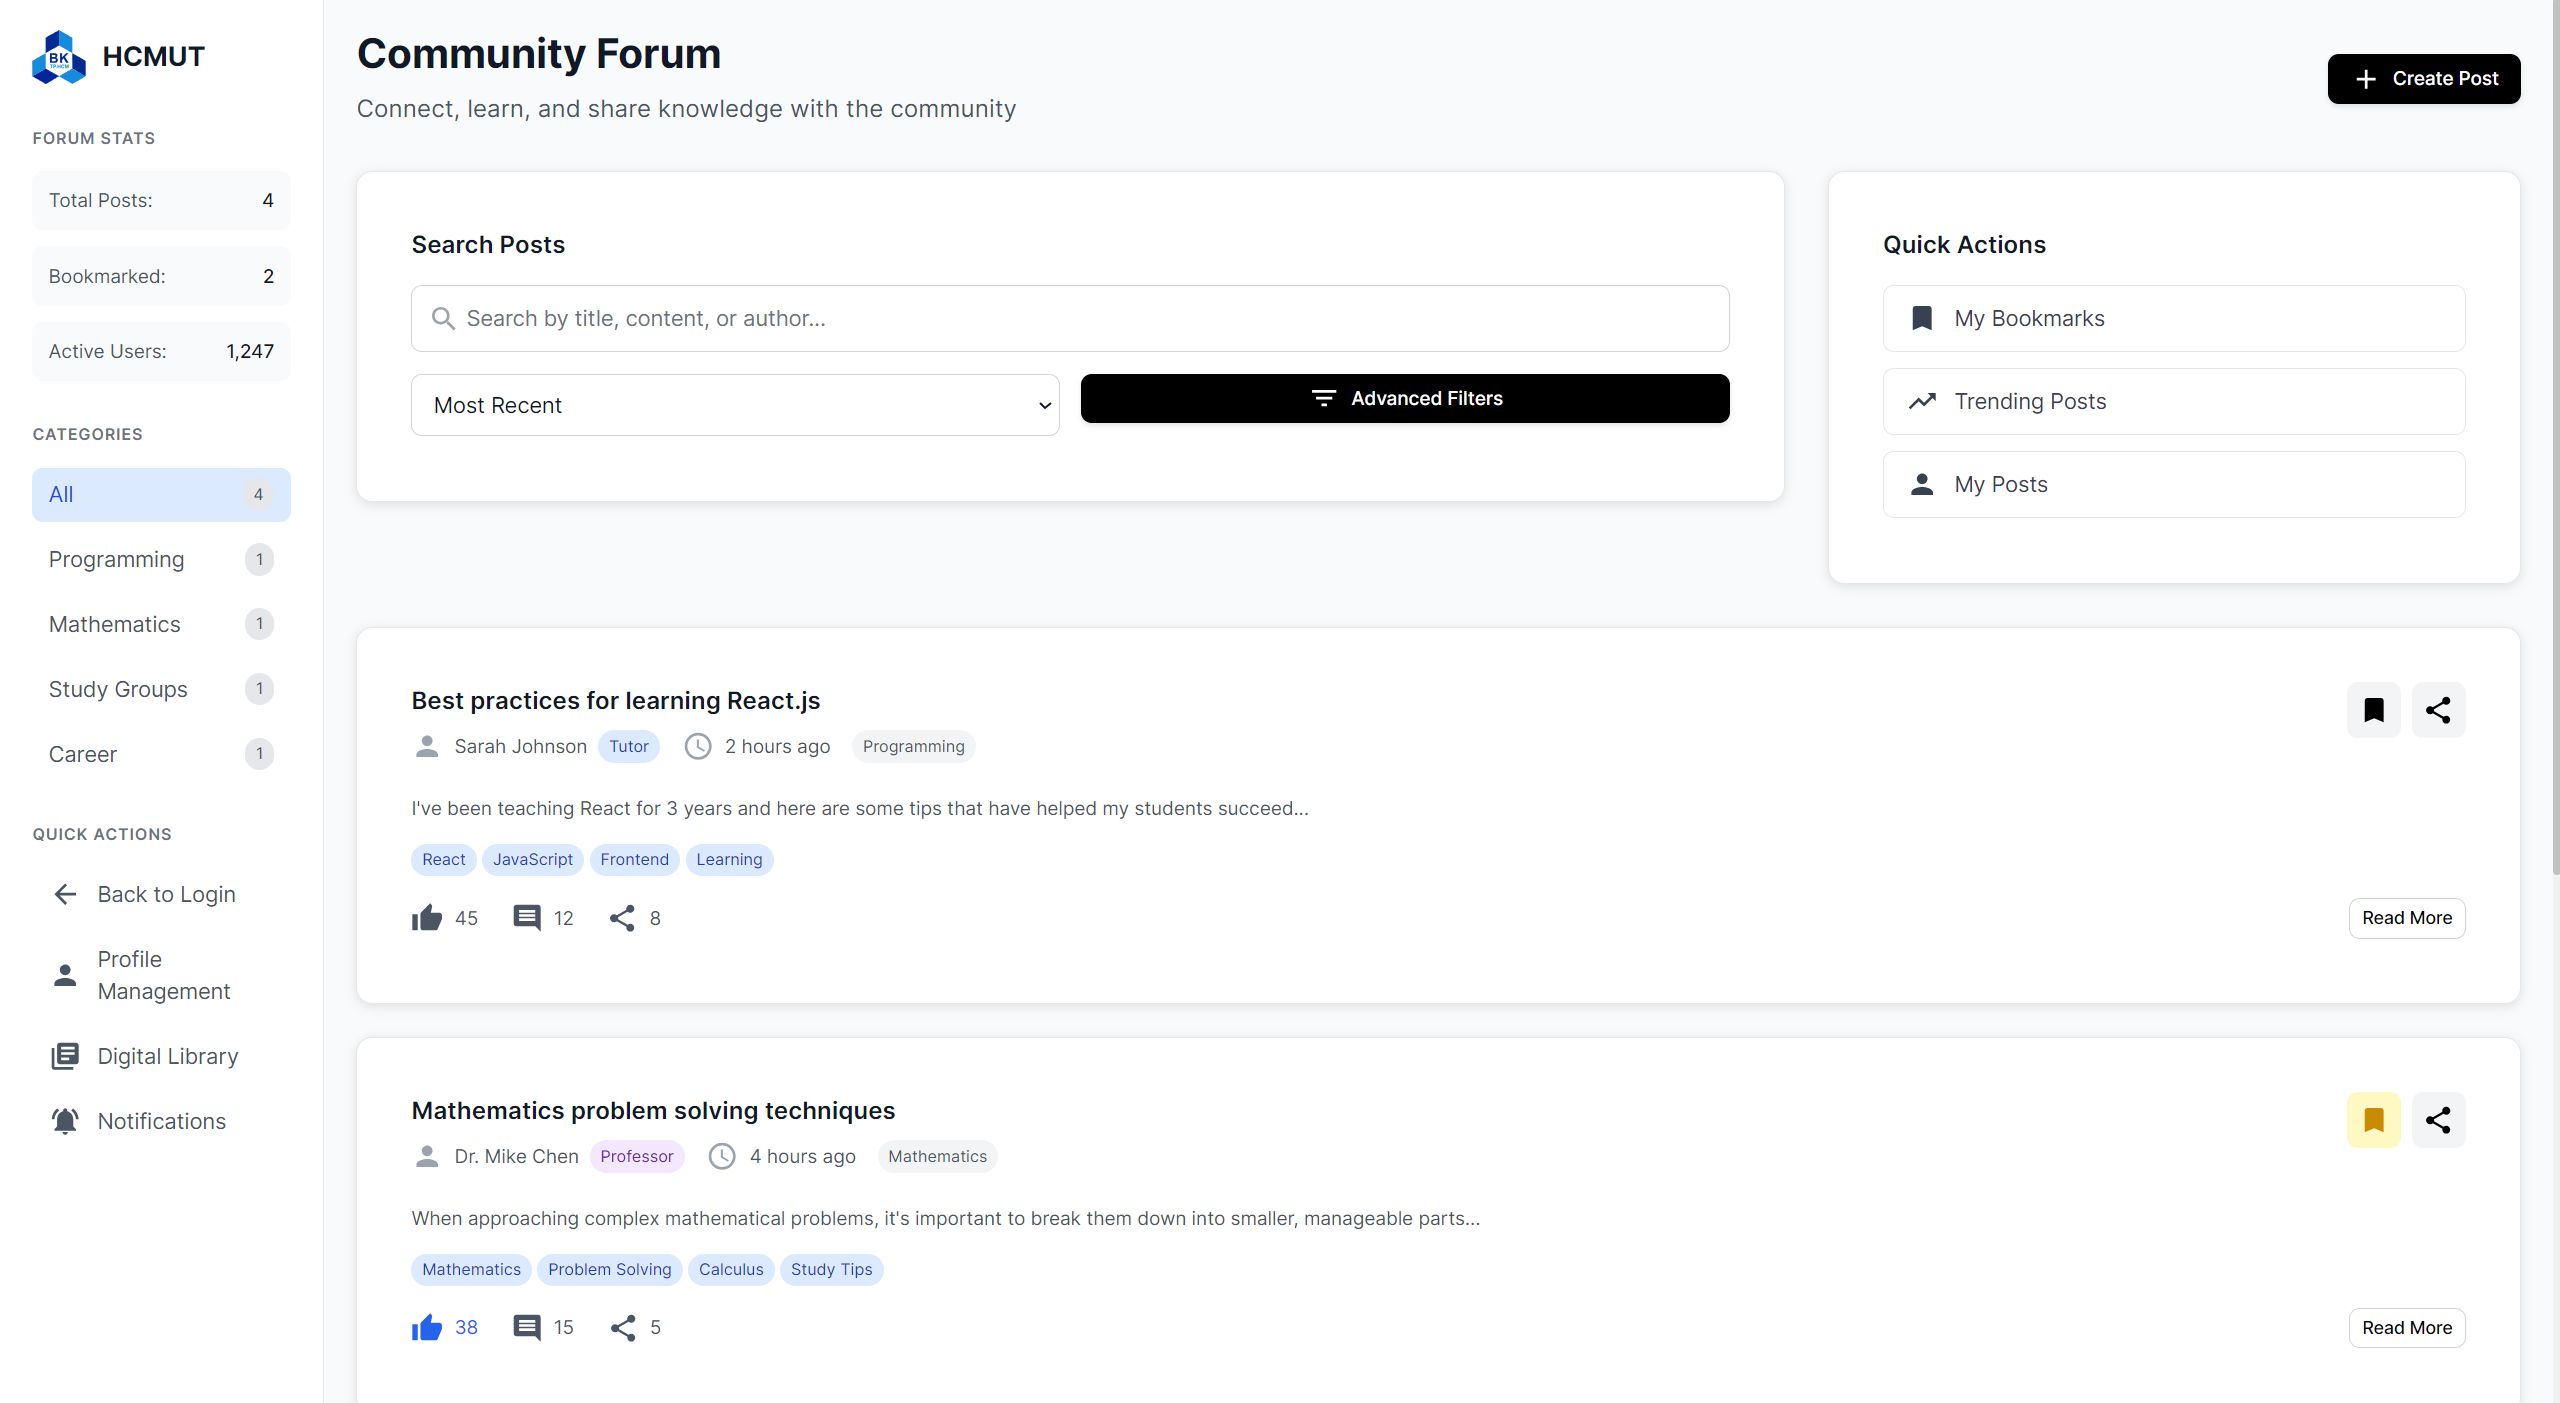
\includegraphics[width=\textwidth]{graphics/chapter2/common/online_community_forum_desktop_overall.png}
    \caption{Online Community Forum Page Overview (Desktop)}
    \label{fig:online_community_forum_desktop_overall}
\end{figure}

\paragraph{General Overview (Desktop)}
The desktop interface features a clean, modern design with forum statistics, search functionality, and post listings.

\subsubsection{Notifications Center}

\noindent The "Notifications Center" page provides users with a centralized hub to view, manage, and filter all their alerts and updates from the platform.

\begin{figure}[H]
    \centering
    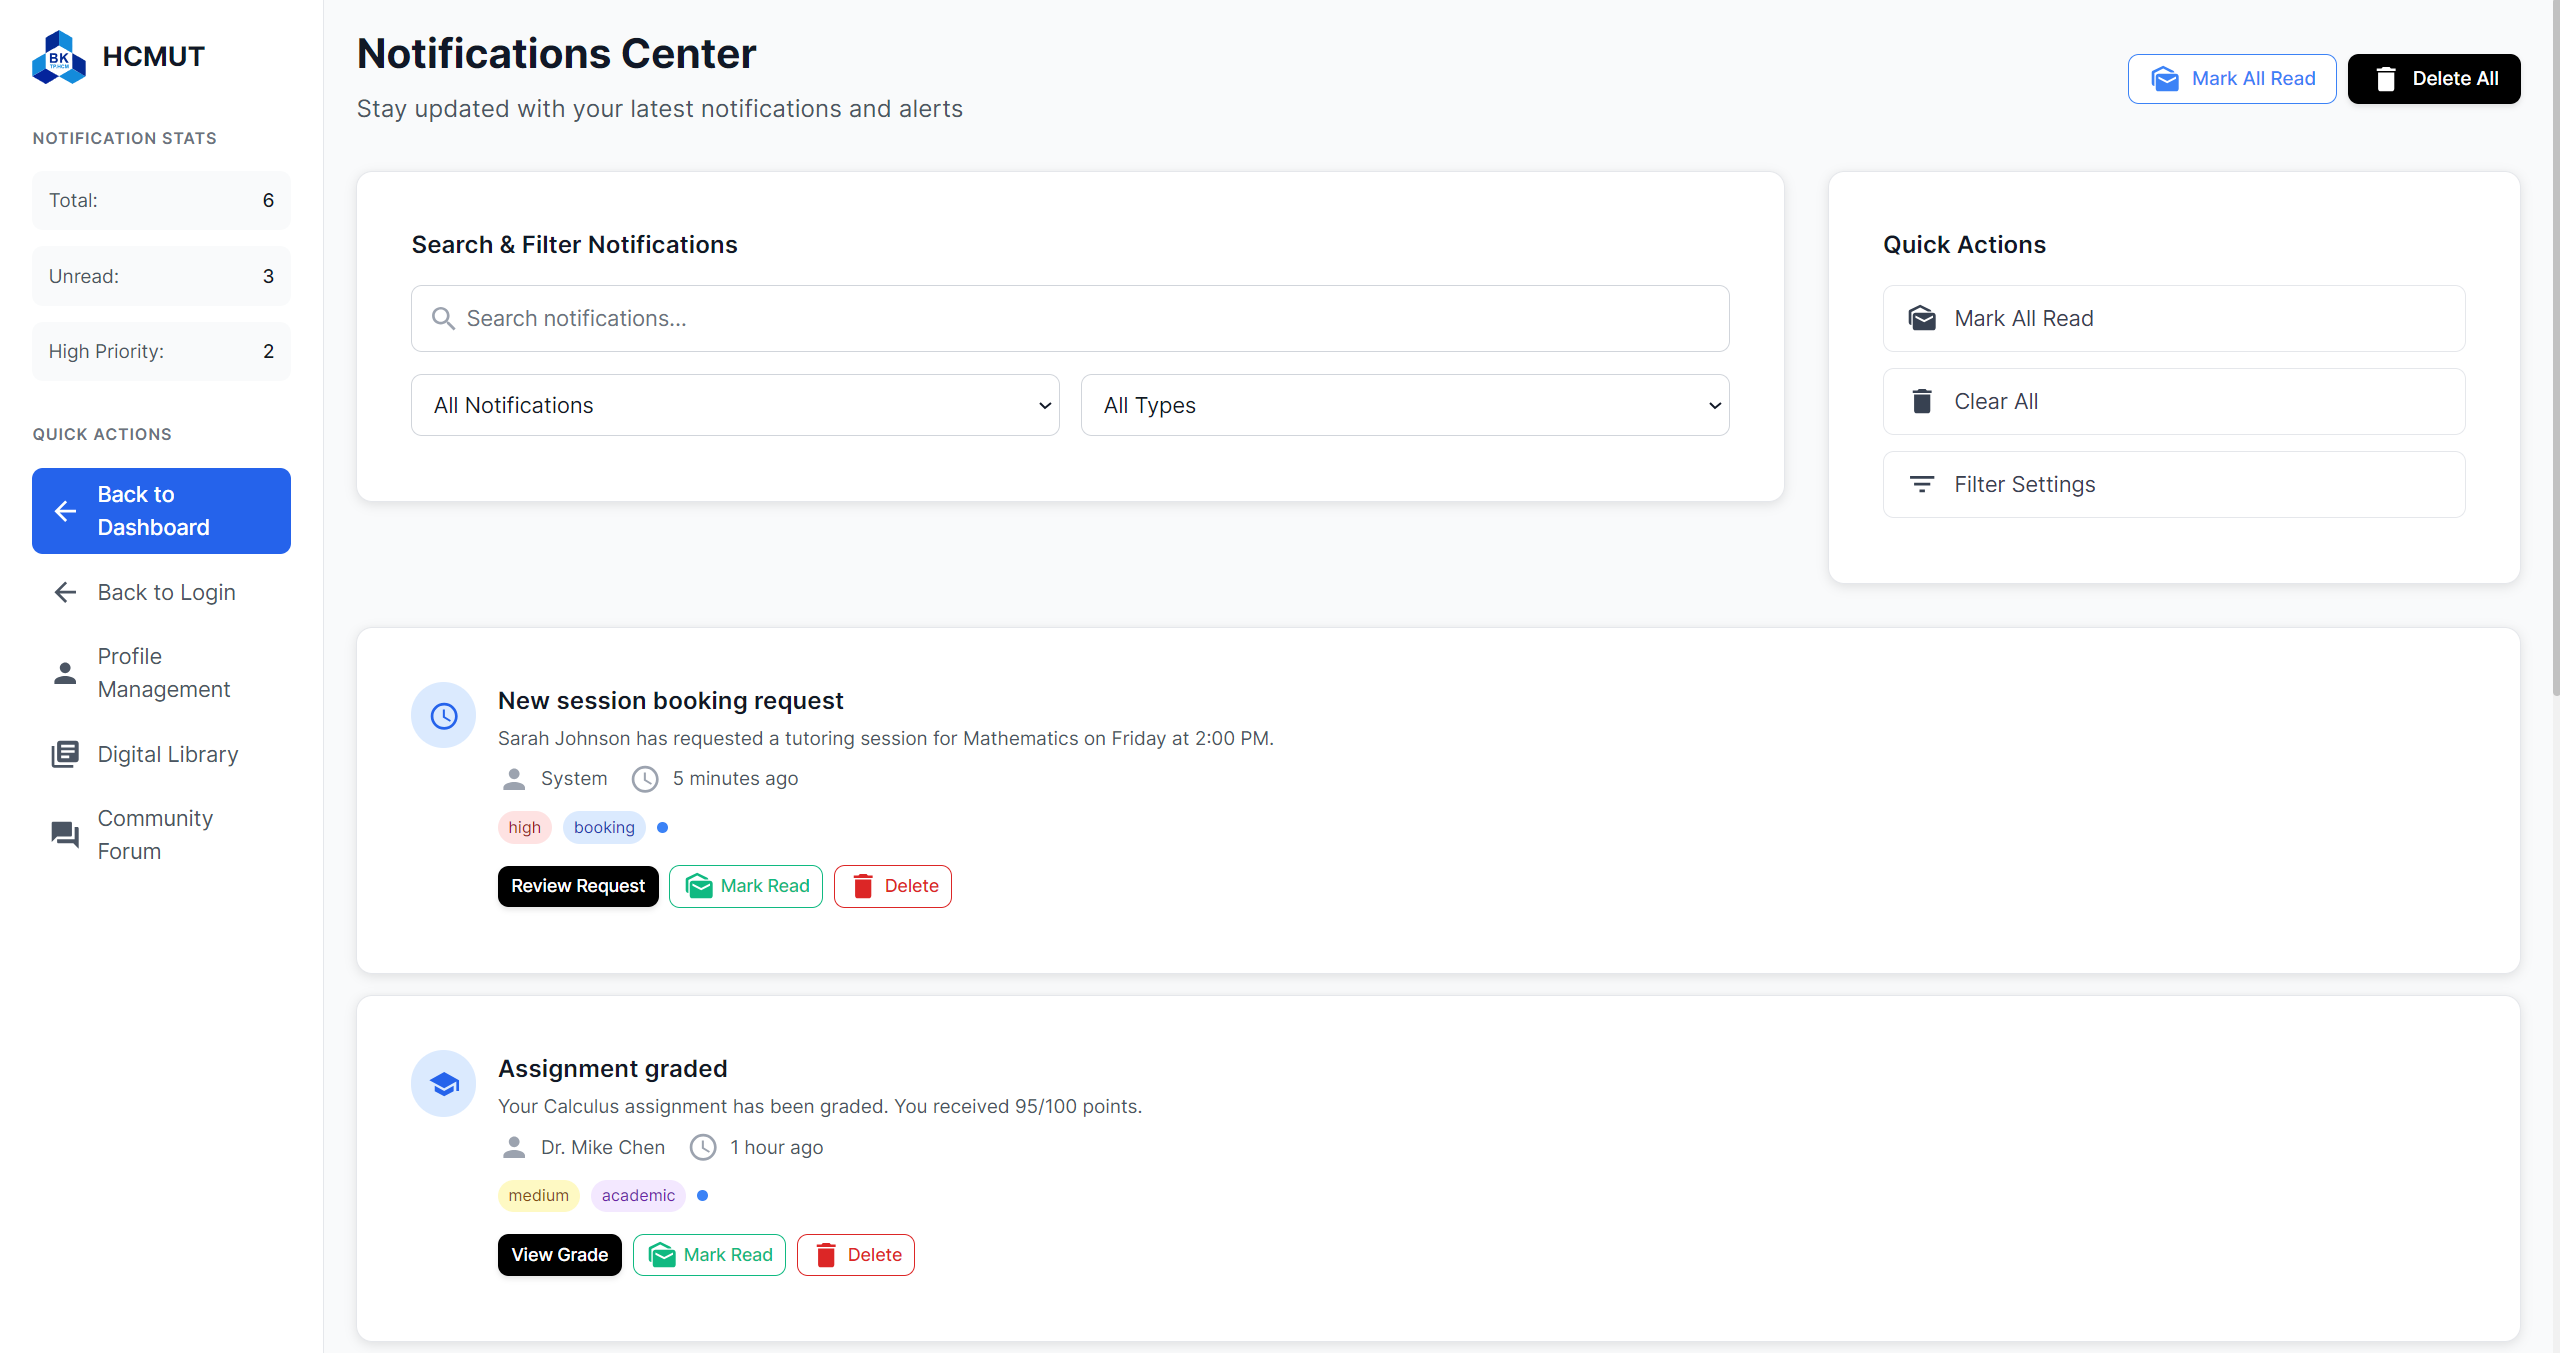
\includegraphics[width=\textwidth]{graphics/chapter2/common/notifications_center_desktop_overall.png}
    \caption{Notifications Center Page Overview (Desktop)}
    \label{fig:notifications_center_desktop_overall}
\end{figure}

\paragraph{General Overview (Desktop)}
The desktop interface features a clean, modern design with notification statistics, search functionality, and individual notification cards.

\subsubsection{Messages}

\noindent The "Messages" page provides users with a centralized communication hub to interact with tutors, students, or other platform users. It features a clear interface for managing conversations and engaging in real-time chat.

\begin{figure}[H]
    \centering
    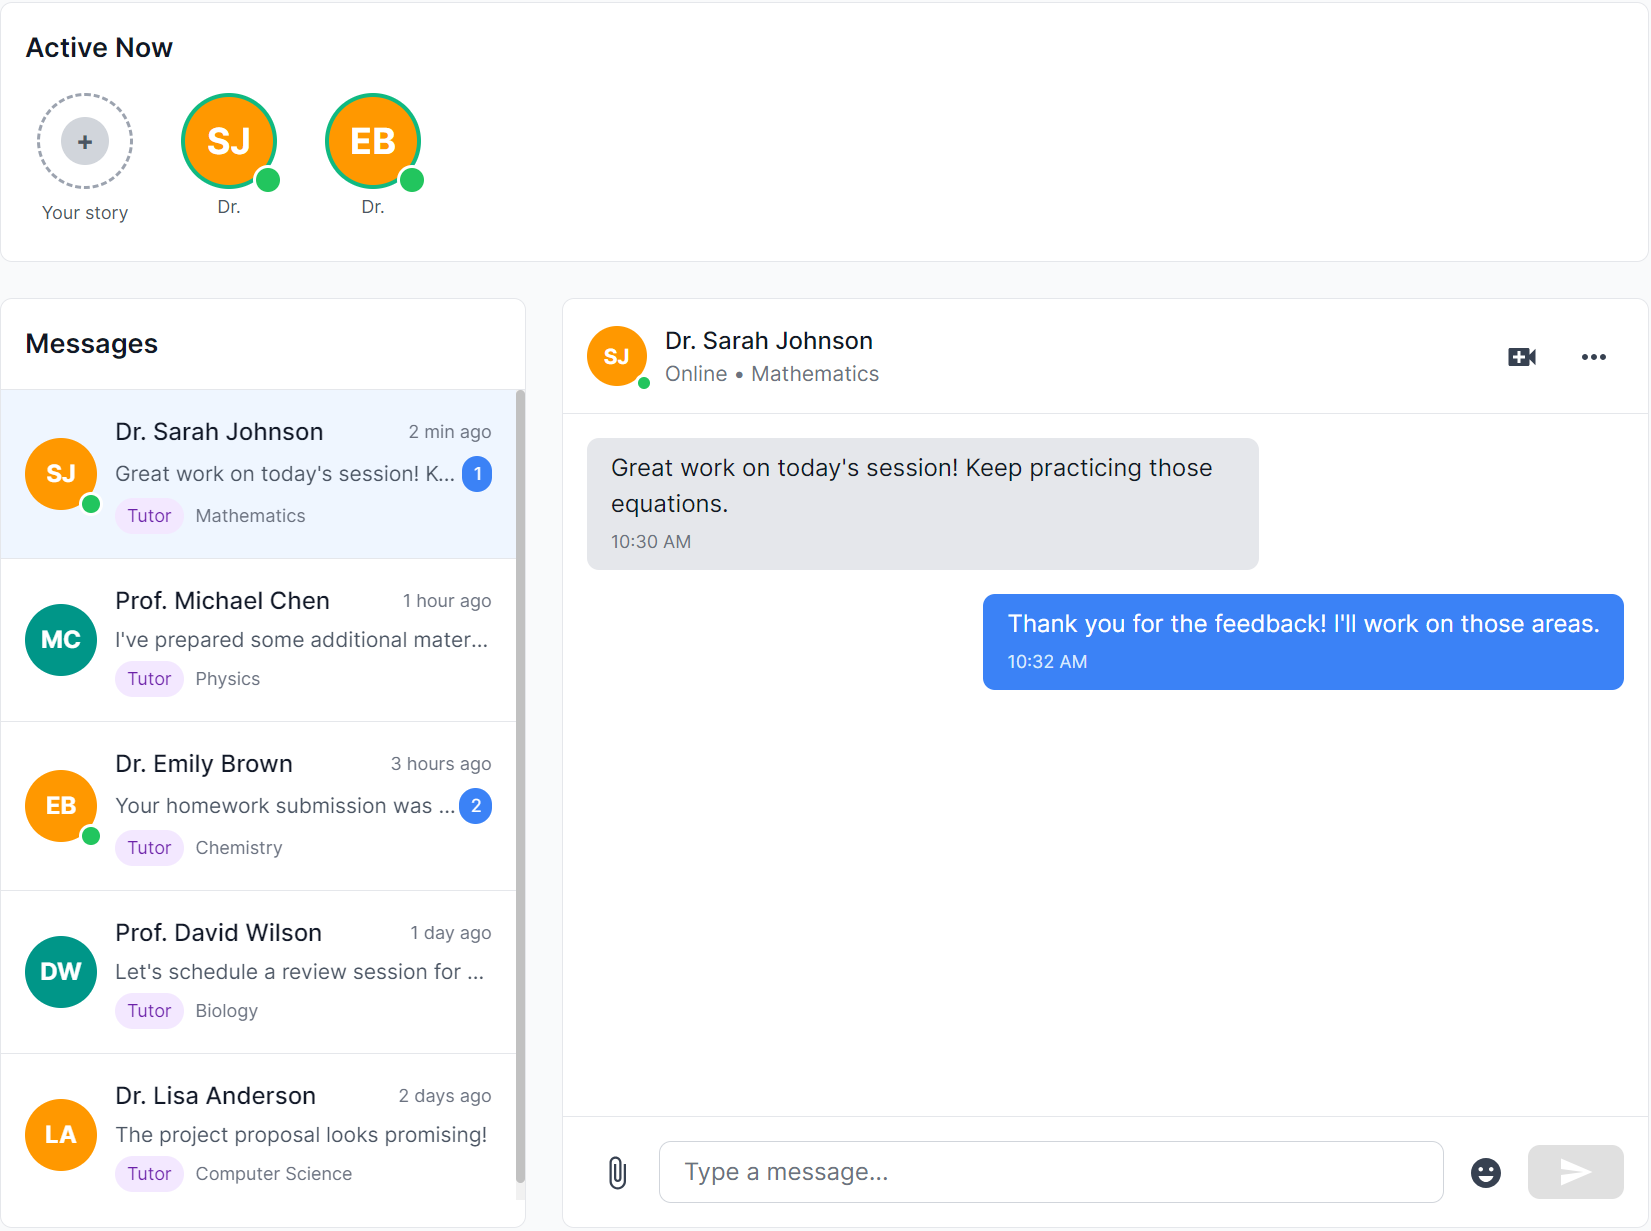
\includegraphics[width=\textwidth]{graphics/chapter2/common/messages_desktop_overall.png}
    \caption{Messages Page Overview (Desktop)}
    \label{fig:messages_desktop_overall}
\end{figure}

\paragraph{General Overview (Desktop)}
The desktop interface features a two-column layout: a left panel for the message list and a right panel for the active chat conversation.

\subsubsection{Calendar}

\noindent The "Calendar" page provides users with a comprehensive view of their scheduled sessions and events, allowing for easy management and navigation through different time perspectives (day, week).

\paragraph{Desktop Interface}
The desktop interface offers a clear and organized layout for viewing and managing events.

\begin{figure}[H]
    \centering
    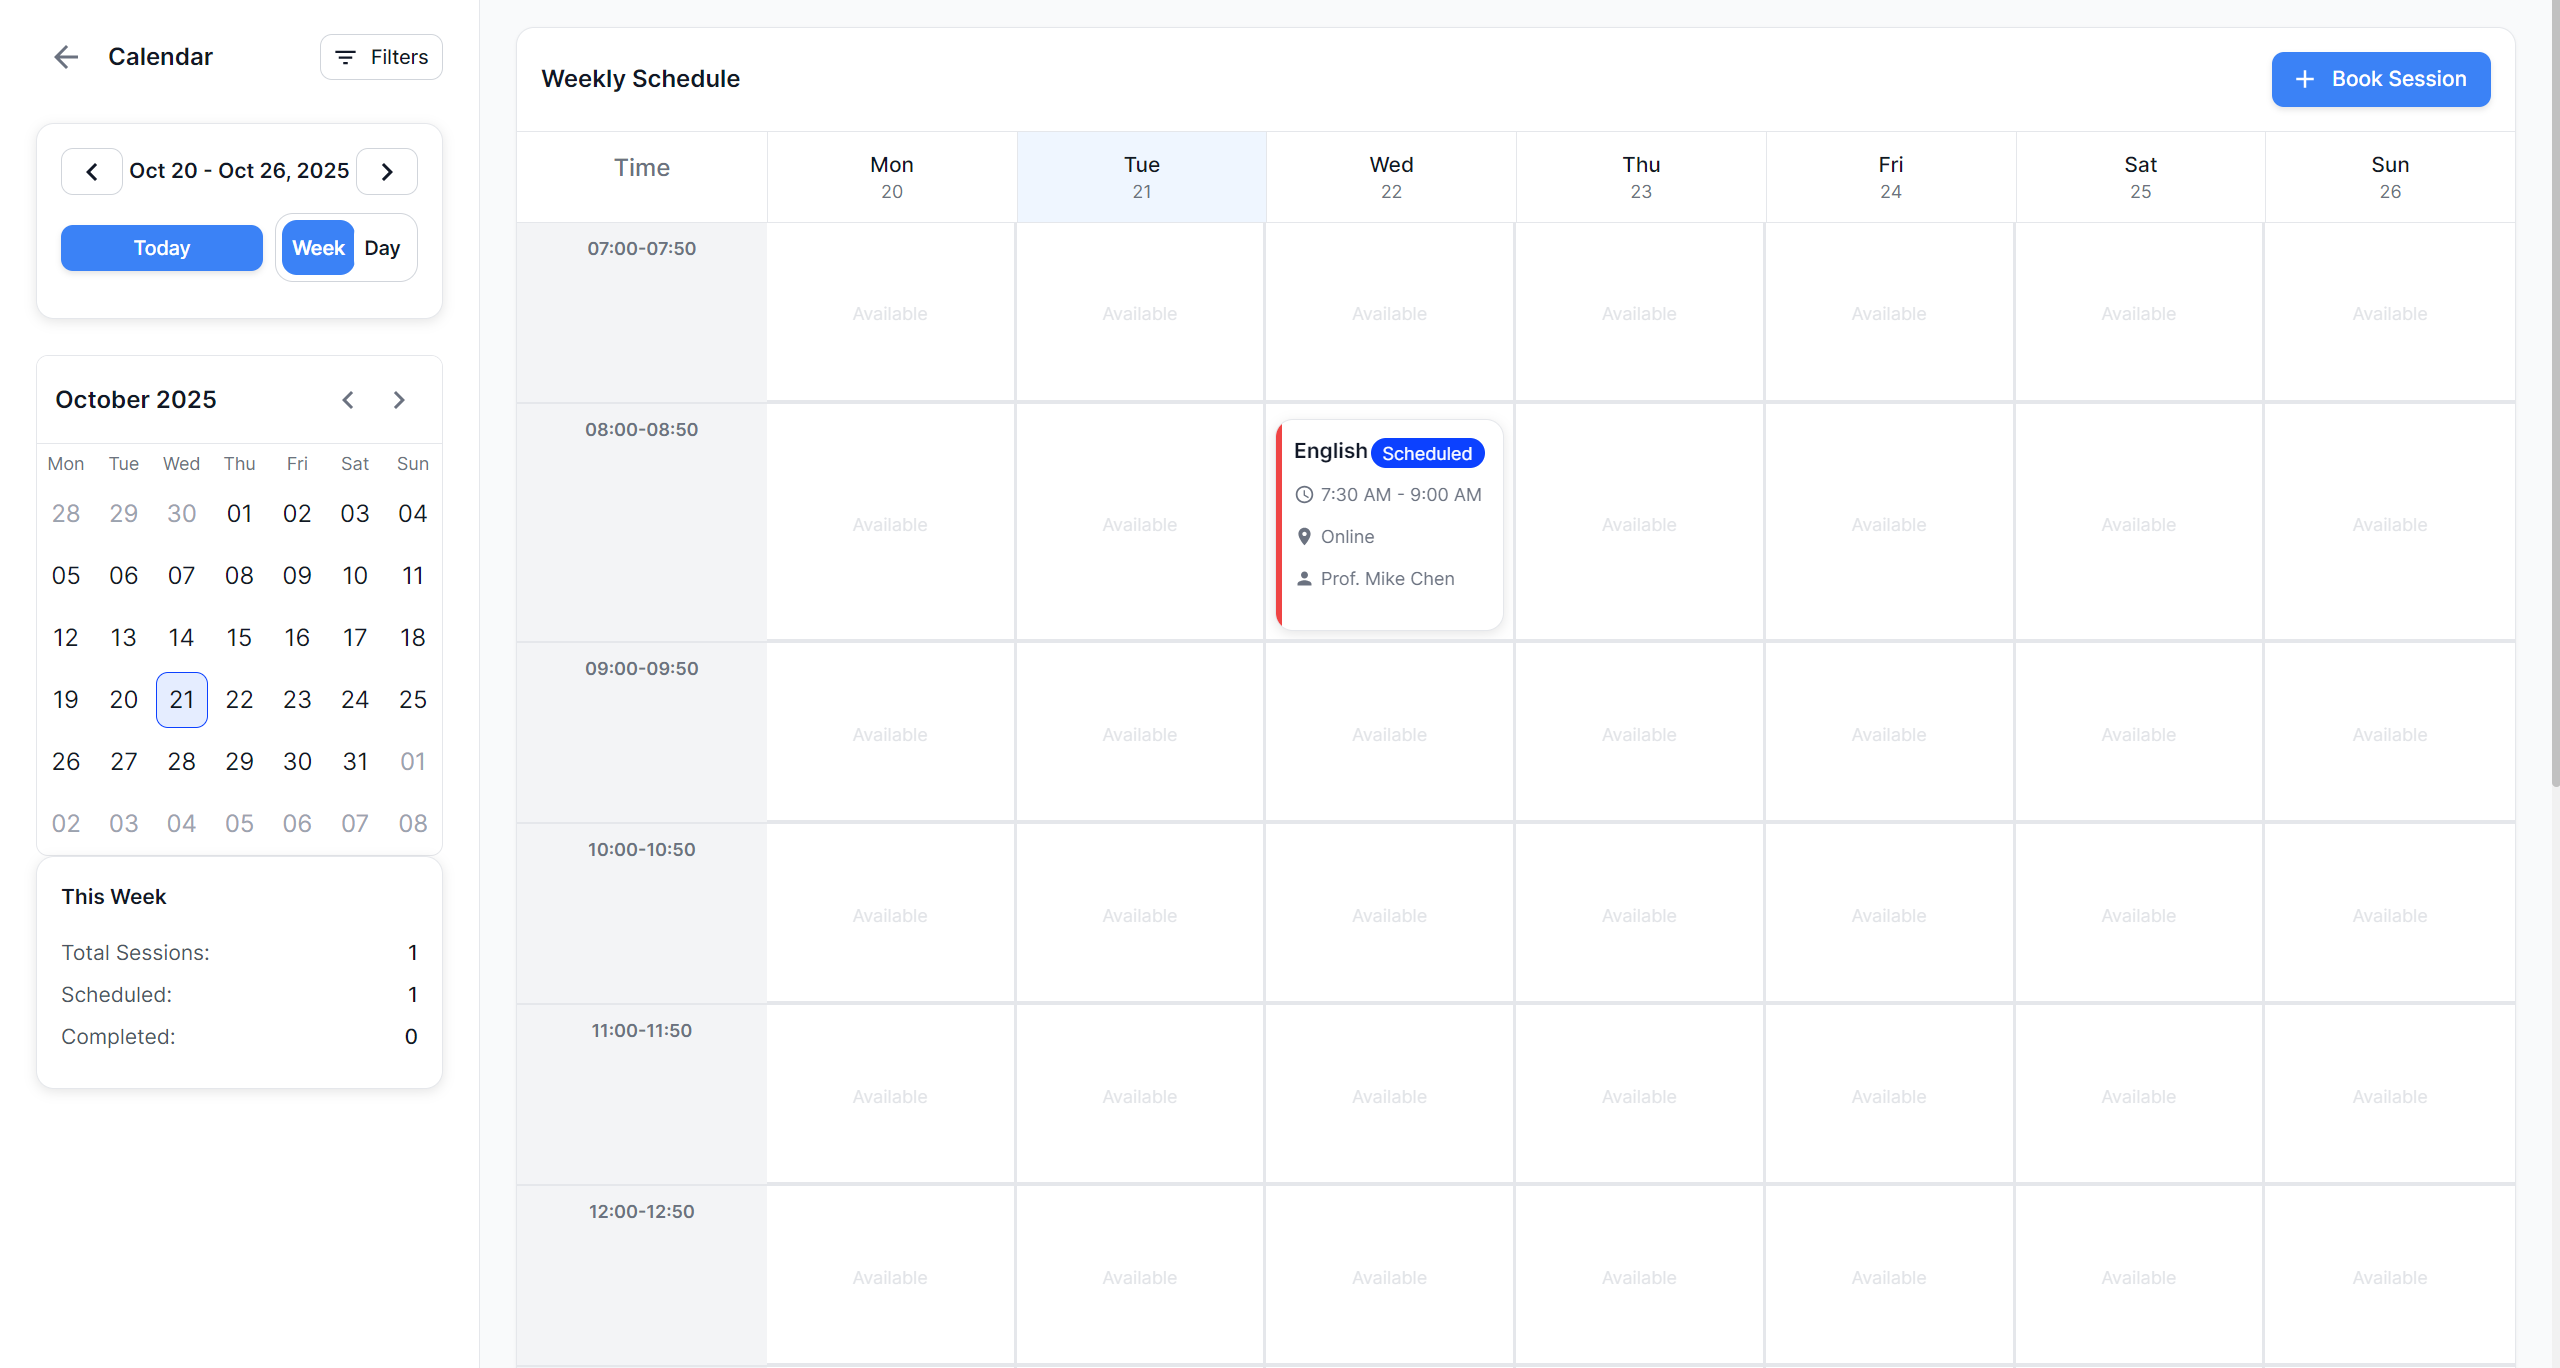
\includegraphics[width=\textwidth]{graphics/chapter2/common/calendar_desktop_week_view.png}
    \caption{Calendar Week View (Desktop)}
    \label{fig:calendar_desktop_week_view}
\end{figure}

\paragraph{Week View (Desktop)}
The week view provides an overview of the entire week's schedule, allowing users to see multiple days at a glance with navigation controls and session cards.

\begin{figure}[H]
    \centering
    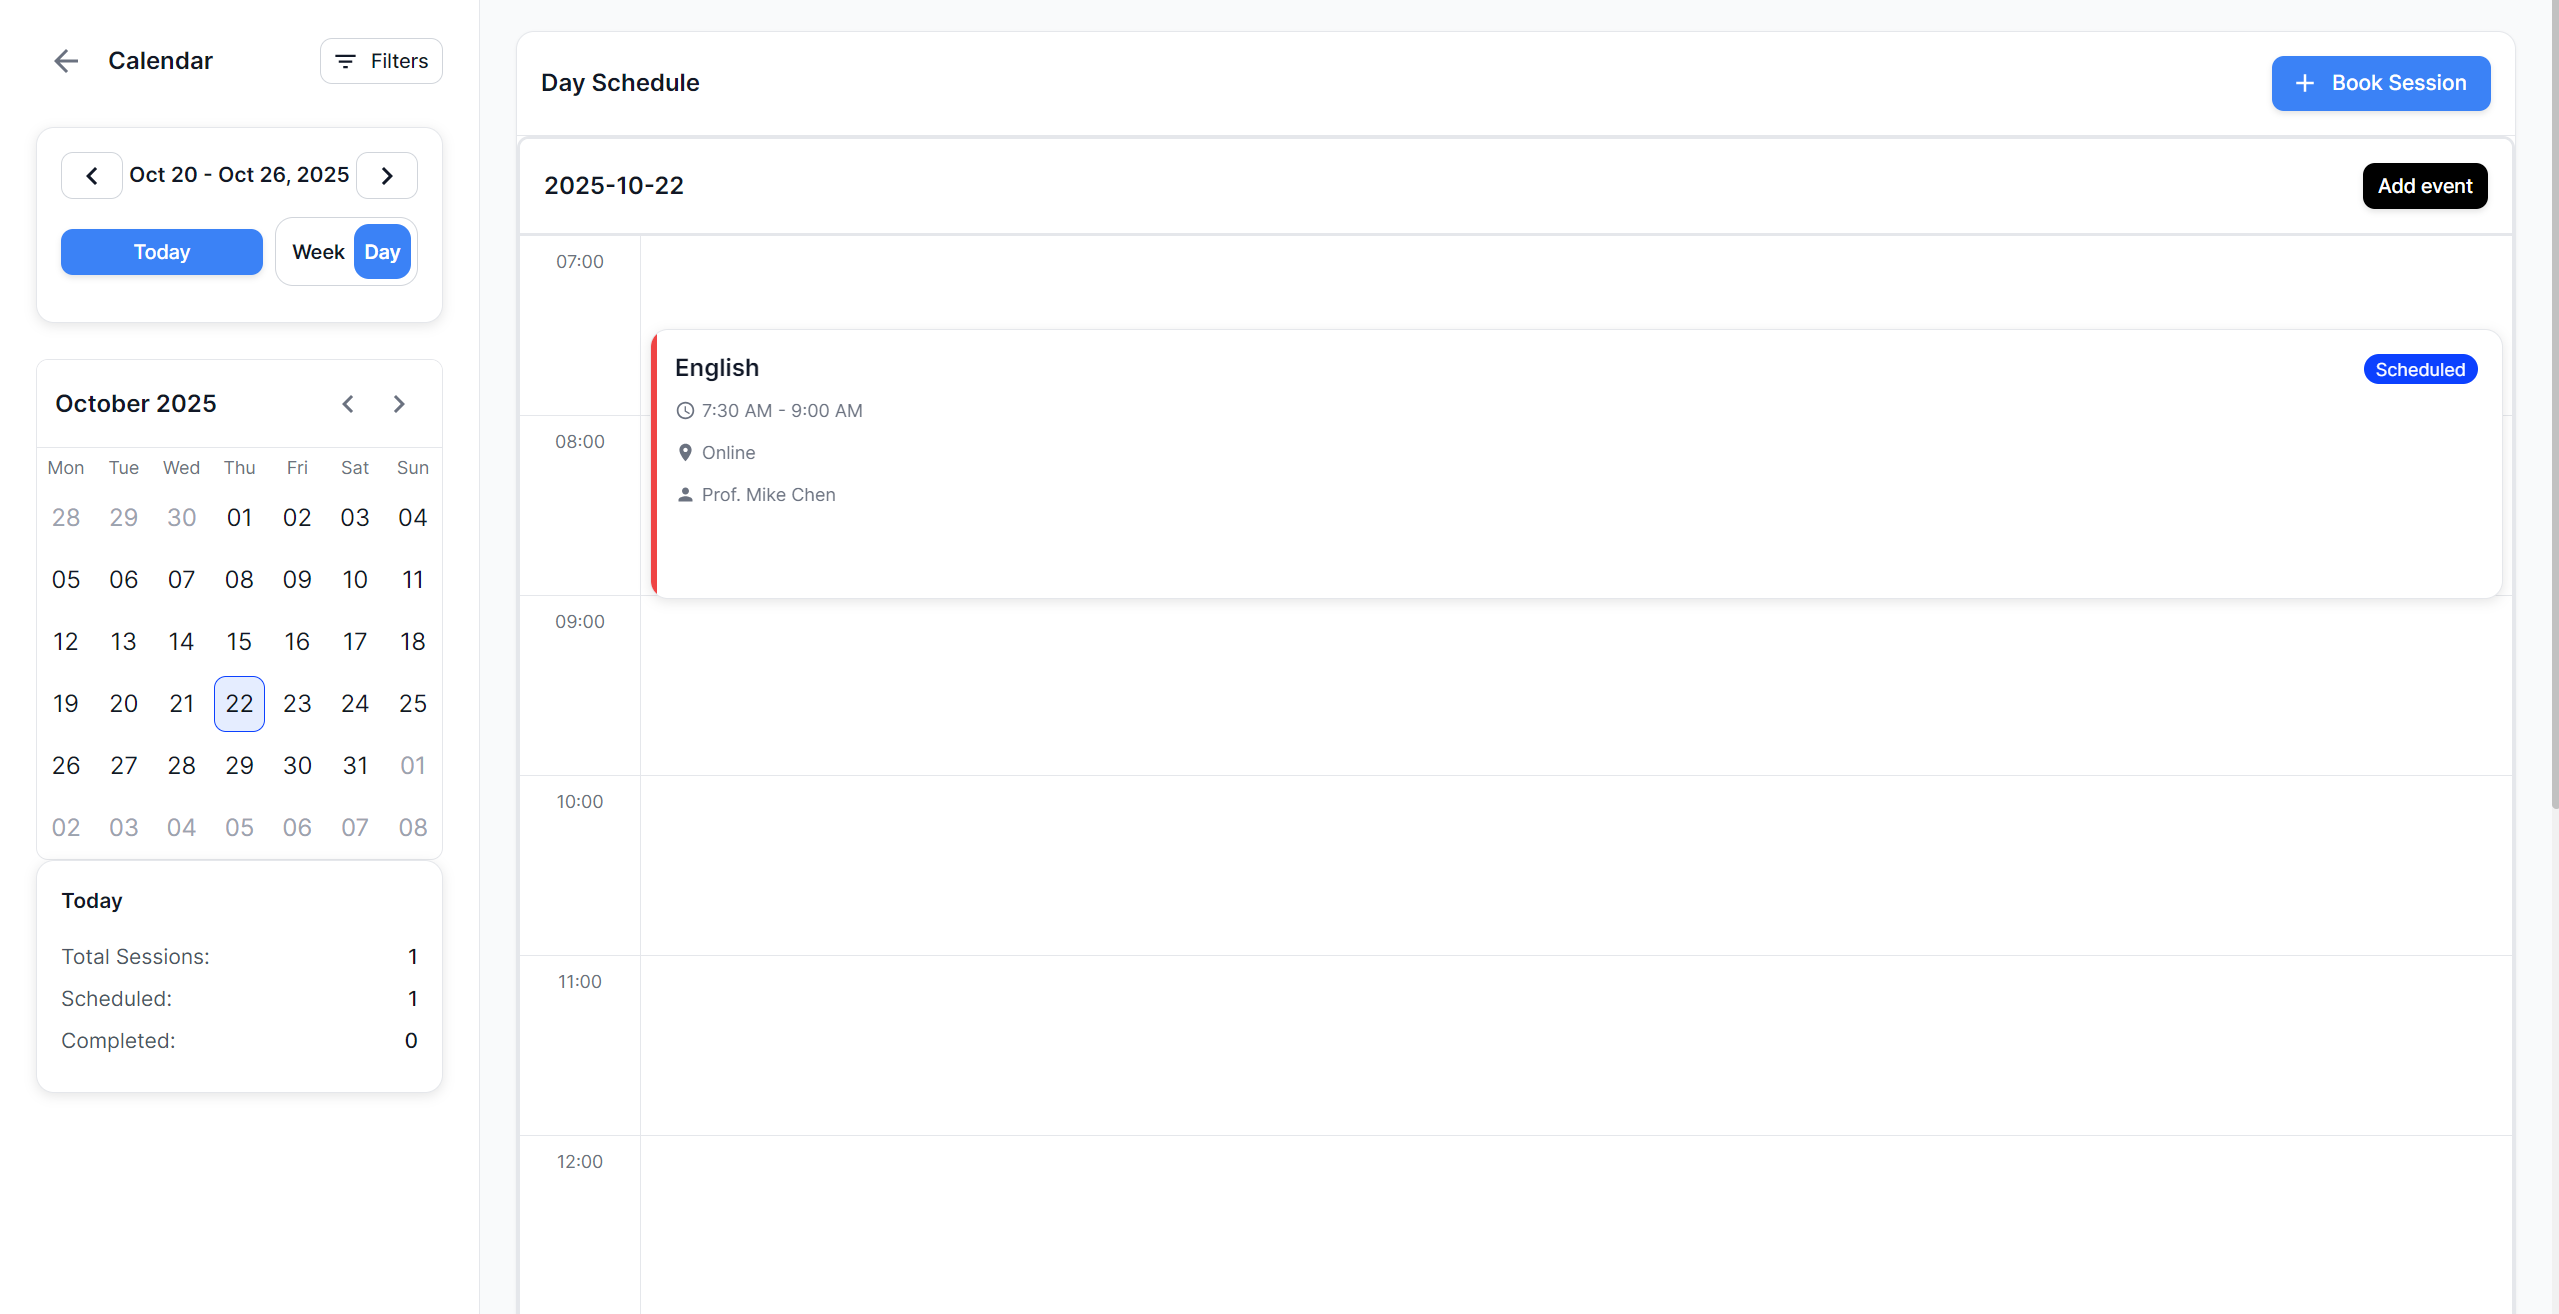
\includegraphics[width=\textwidth]{graphics/chapter2/common/calendar_desktop_day_view.png}
    \caption{Calendar Day View (Desktop)}
    \label{fig:calendar_desktop_day_view}
\end{figure}

\paragraph{Day View (Desktop)}
The day view displays a single day's schedule, showing time slots and detailed event cards with navigation for weeks and view toggles.
